\documentclass[10pt,a4paper]{article}
%\documentclass[10pt,twocolumn,a4paper]{article}

\usepackage{amsmath, amssymb, braket}
\usepackage{graphicx}
\usepackage{subfig}
\usepackage{a4wide}
\usepackage[lined]{algorithm2e}
\usepackage[colorlinks]{hyperref}
\usepackage{parcolumns}
\usepackage{mathpazo}

\newcommand{\CCS}{{\tt CCS}}
\newcommand{\CCSCode}[1]{{\tt #1}}

\newcommand{\Agent}[1]{{\tt {#1}}}
\newcommand{\Action}[1]{{\tt \bf {#1}}}
\newcommand{\CoAction}[1]{$\overline{\mbox{\Action{#1}}}$}

\newcommand{\FileName}[1]{{\sf {#1}}}

\setlength{\parindent}{0pt}
\setlength{\parskip}{2ex}

\title {
    Concurrency Theory Project
}
\author{
    Giovanni Simoni\\
    Register 142955\\
    \href{mailto:giovanni.simoni@roundhousecode.com}
         {giovanni.simoni@roundhousecode.com}
}

\begin{document}

\maketitle

\section{Introduction}

    I chose to implement the first project, namely the \emph{Dekker}
    protocol for mutual exclusion.

    My implementation aims to be as modular as possible by extensively
    using the parametrization of \CCS{} entities.

    The technique consists in defining abstract behaviors in terms of
    agents, whose actions are binded by formal parameters. Instantiation
    of an abstract behavior into a concrete process consists in the
    definition a new agent which parametrizes the abstract one with
    variables used by other processes.

    In order to obtain a more visually straightforward representation of
    the formal definitions, in this document I shall omit the formal
    parameters for actions: the complete definition can be read in the
    \FileName{dekker.ccs} file, coming along with this report.

\section{The protocol}

    The implementation encodes two abstract behaviors:

    \begin{itemize}

    \item   The read/write behavior of boolean variables, which values can
            be read or re-assigned by means of actions (see
            Picture~\ref{pic:Bool}).

    \item   The sequence of actions specified by the Dekker
            protocol (see Picture~\ref{pic:Dekker});

    \end{itemize}

    \begin{figure}[htbp]
        \centering
        \subfloat[Boolean variable process]{
            \label{pic:Bool}
            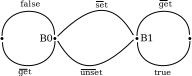
\includegraphics[width=.5\textwidth]{pics/bool}
        }
        \subfloat[Dekker process]{
            \label{pic:Dekker}
            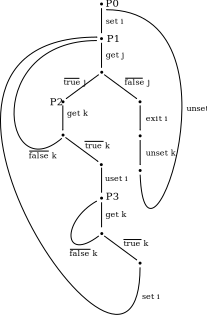
\includegraphics[width=.5\linewidth]{pics/dekker}
        }

        \label{pic:Protocol}
        \caption{The graph of abstract behaviors. The left graph shows the
                 encoding of a process implementing the Dekker
                 protocol, while the right one shows the behavior of a
                 process emulating a boolean variable.}

    \end{figure}

    \subsection{Encoding of the boolean variable abstraction}
    \label{sub:EncodeBool}

        The variable consists in two main processes:

        \begin{verbatim}
agent B0 = 'set.B1 + 'get.false.B0;
agent B1 = 'unset.B0 + 'get.true.B1;
        \end{verbatim}

        \begin{itemize}

        \item   \Agent{B0} models the behavior of a boolean variable
                initialized to False. It can be queried with a
                \CoAction{get} action (the \Action{false} action will be
                produced) or setted to True by a \CoAction{set} action
                (the \Agent{B1} behavior will be assumed);

        \item   \Agent{B1} is the dual of \Agent{B0}, and models the
                behavior of a false boolean variable 
                to True. As for \Agent{B0} it can be queried with a
                \CoAction{get} action (the \Action{true} action will be
                produced instead) or setted to False by a \CoAction{unset}
                action (the \Agent{B0} behavior will be assumed).

        \end{itemize}

    \subsection{Encoding of the Dekker protocol abstraction}

        \subsubsection{Branching points}
        \label{subsub:BranchingPoints}

            In order to encode the protocol I simply considered the
            \emph{branching points} of the given algorithmic version of
            the protocol, and converted them into \CCS{} \emph{choice
            operators}.

            \noindent For instance, an \emph{if-then-else} like
            \begin{quote}
                \begin{algorithm}[H]
                \eIf{$x$}{
                    $y$ $\leftarrow$ true;
                }{
                    $y$ $\leftarrow$ false;
                }
                \end{algorithm}
            \end{quote}
            can be represented as
            \begin{quote}
            \CCSCode{getx.('xtrue,.sety + 'xfalse.unsety)}
            \end{quote}
            where
            \begin{itemize}

            \item   \CCSCode{getx} is the output action querying for the
                    value of $x$;

            \item   \CCSCode{'xtrue} and \CCSCode{'xfalse} are the input
                    actions required to read respectively \emph{true} or
                    \emph{false} as result of the \CCSCode{getx} query;

            \item   \CCSCode{sety} and \CCSCode{unsety} are the output
                    actions used respectively to set to \emph{true} or
                    \emph{false} the $y$ variable.

            \end{itemize}

        \subsubsection{The actual code}

            The protocol requires: two boolean variables $b_i$ and $b_j$
            for critical section access request plus an integer variable
            $k$ representing the turn. Since however $k$ can take values in
            $\Set{0, 1}$, I simply considered it as it were a boolean
            variable as well

            For convenience the protocol has been split into four
            processes: the first one is the starting point of the
            protocol's main loop, while the others are mapped on the three
            branching point of the algorithm.

            According to what explained in Subsection~\ref{sub:EncodeBool}
            and following the naming conventions showed in
            Paragraph~\ref{subsub:BranchingPoints}, the abstract behavior
            is encoded as follows:
\begin{verbatim}
agent P0 = seti.P1;
agent P1 = getj.( 'truej.P2 + 'falsej.exiti.unsetk.unseti.P0 );
agent P2 = getk.( 'falsek.P1 + 'truek.unseti.P3 );
agent P3 = getk.( 'falsek.P3 + 'truek.seti.P1 );
\end{verbatim}

\end{document}
